\documentclass[a4paper,12pt]{article}

\usepackage[utf8]{inputenc}
\usepackage[T1]{fontenc}
\usepackage[portuguese]{babel}
\usepackage{amsmath}
\usepackage{booktabs}
\usepackage{graphicx}
\usepackage{subcaption}
\usepackage{geometry}
\usepackage{xcolor}
\usepackage{listings}
\usepackage{pgfplots}
\pgfplotsset{compat=1.16}
\geometry{margin=2.5cm}

\graphicspath{{imagens/}}

\definecolor{codebg}{RGB}{245,245,245}
\definecolor{codegray}{RGB}{110,110,110}
\definecolor{codegreen}{RGB}{0,128,0}
\definecolor{codeblue}{RGB}{0,0,200}
\definecolor{codeorange}{RGB}{200,90,0}

\lstdefinestyle{cstyle}{
    backgroundcolor=\color{codebg},
    commentstyle=\color{codegreen}\itshape,
    keywordstyle=\color{codeblue}\bfseries,
    stringstyle=\color{codeorange},
    numberstyle=\tiny\color{codegray},
    basicstyle=\ttfamily\footnotesize,
    breakatwhitespace=false,
    breaklines=true,
    captionpos=b,
    keepspaces=true,
    numbers=left,
    numbersep=8pt,
    showspaces=false,
    showstringspaces=false,
    showtabs=false,
    tabsize=4,
    frame=single,
    rulecolor=\color{codegray!40},
    language=C
}

\title{Tarefa 11 - Particionamento de dados e balanceamento de carga}
\author{Israel Soares de Castro Filho \\ Matrícula: 20250070780}
\date{}

\begin{document}

\maketitle

\section{Introdução}

Este relatório apresenta a implementação, em linguagem C, de um simulador de
fluido 2D que resolve a equação de Navier--Stokes considerando \emph{apenas} o
efeito da viscosidade (sem pressão, sem advecção e sem forças externas):

\begin{equation}
    \frac{\partial \mathbf{u}}{\partial t} = \nu \left(
    \frac{\partial^2 \mathbf{u}}{\partial x^2} +
    \frac{\partial^2 \mathbf{u}}{\partial y^2} \right),
    \qquad \mathbf{u} = (u, v).
\end{equation}

Primeiro, o código sequencial é validado: um fluido parado deve permanecer
parado, e uma pequena perturbação deve se difundir suavemente, de acordo com a
solução analítica. Em seguida, o código é paralelizado com OpenMP, e o foco
passa a ser o impacto das cláusulas \texttt{schedule} e \texttt{collapse} no
desempenho, avaliado com o PaScal Suite.

\section{Metodologia}

\subsection{Discretização}

O domínio é o quadrado $[0,1]^2$, com malha uniforme de $N \times N$ células e
contorno periódico nas duas direções. Usa-se diferenças finitas com o esquema
explícito FTCS e estêncil de cinco pontos:

\begin{equation}
    u^{n+1}_{i,j} = u^{n}_{i,j} + r\left(u^{n}_{i+1,j} + u^{n}_{i-1,j} +
    u^{n}_{i,j+1} + u^{n}_{i,j-1} - 4u^{n}_{i,j}\right),
    \qquad r = \frac{\nu\,\Delta t}{\Delta x^2},
\end{equation}

e equação análoga para $v$. O método é estável em 2D para $r \le 0{,}25$; o
código fixa $r = 0{,}2$ e calcula $\Delta t$ a partir dele.

\subsection{Casos de teste}

\begin{itemize}
    \item \textbf{Fluido parado} ($u = v = 0$): o campo deve permanecer nulo.
    \item \textbf{Perturbação gaussiana} em $u$, com $A = 1$ e
    $\sigma_0 = 0{,}05$, centrada em $(0{,}5;\,0{,}5)$. Para uma gaussiana 2D,
    a difusão pura tem solução analítica na qual o pico decai como
    \begin{equation}
        u_{\max}(t) = \frac{A\,\sigma_0^2}{\sigma_0^2 + 2\nu t}.
    \end{equation}
\end{itemize}

\subsection{Paralelização e experimento de desempenho}

O passo de tempo foi paralelizado em duas versões do mesmo kernel, apresentadas
no Apêndice~\ref{ap:codigo}:

\begin{itemize}
    \item \textbf{\texttt{schedule(static)}}: \texttt{parallel for} apenas no
    laço externo (\texttt{i}), com escalonamento estático;
    \item \textbf{\texttt{collapse(2)}}: os laços \texttt{i} e \texttt{j} são
    fundidos em um espaço de $N^2$ iterações, também com escalonamento estático.
    Como o \texttt{collapse} exige laços perfeitamente aninhados, o cálculo dos
    vizinhos periódicos (\texttt{im}, \texttt{ip}) passa para dentro do corpo e é
    refeito a cada ponto.
\end{itemize}

No experimento de desempenho, a malha foi fixada em $N = 1024$ e o único
parâmetro de entrada foi o tempo final $t_{final}$. As entradas i1 a i4
dobram o tempo simulado a cada passo, de modo que o trabalho total também dobra. 
As execuções foram feitas com o PaScal Analyzer, com instrumentação manual da região do passo
de tempo, para 1, 2, 4 e 8 cores. O PaScal Viewer calcula o speedup de cada
versão em relação à \emph{sua própria} execução com 1 core.

\section{Validação do código}

\subsection{Fluido parado}

A Figura~\ref{fig:sim0} mostra a simulação de um fluido inicialmente parado
($N = 128$, $\nu = 0{,}05$, até $t = 2$). Nos quatro instantes exibidos o campo
é uniforme e igual a zero, o perfil central $u(x, y = L/2)$ coincide com $u = 0$
em todos os tempos e o máximo de $u$ permanece nulo ao longo de toda a
simulação. Como o laplaciano de um campo nulo é nulo, esse é o resultado
esperado. O teste indica que o esquema não gera velocidade espúria.

\begin{figure}[ht]
    \centering
    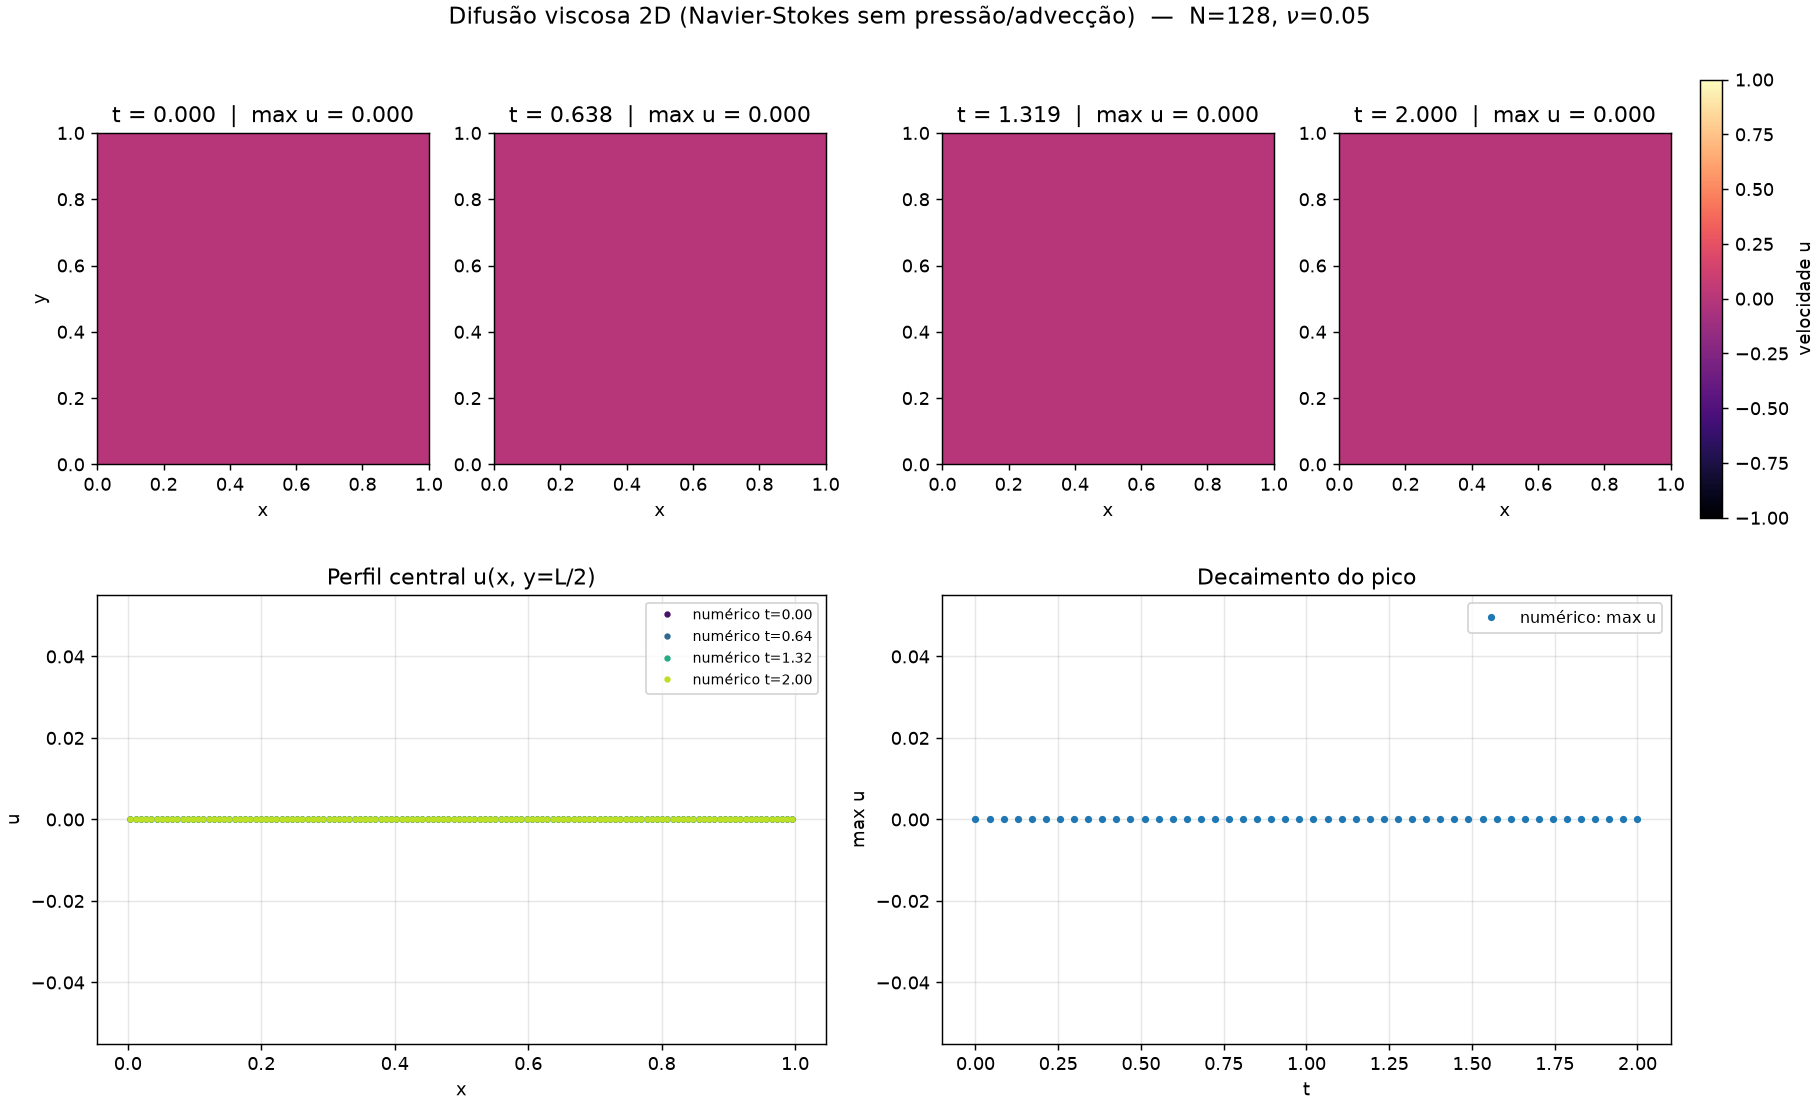
\includegraphics[width=\linewidth]{../ground_truth/simulacao0/difusao_figura.png}
    \caption{Fluido parado ($N=128$, $\nu = 0{,}05$): o campo permanece nulo.}
    \label{fig:sim0}
\end{figure}

\subsection{Difusão de uma perturbação}

A Figura~\ref{fig:sim1} mostra a difusão da perturbação gaussiana
($N = 128$, $\nu = 0{,}01$, até $t = 0{,}5$). Os mapas de calor mostram o pico
se alargando e perdendo intensidade, sem oscilações nem artefatos nas bordas. O
máximo de $u$ cai de $0{,}994$ em $t = 0$ para $0{,}437$, $0{,}275$ e $0{,}200$
em $t = 0{,}160$, $0{,}329$ e $0{,}500$. Esses valores coincidem com a
expressão analítica: para $t = 0{,}5$ e $\nu = 0{,}01$,
$0{,}0025/(0{,}0025 + 0{,}01) = 0{,}200$, e para $t = 0{,}329$ obtém-se
$\approx 0{,}275$. Os perfis centrais numéricos também ficam sobre as curvas
analíticas, e a curva de decaimento do pico segue a previsão ao longo de todo o
intervalo.

O valor inicial de $0{,}994$, e não $1{,}0$, não é um erro: com $N = 128$ par,
nenhum centro de célula coincide exatamente com o centro da gaussiana, e o pico
é amostrado a meia célula de distância em cada direção.

\begin{figure}[ht]
    \centering
    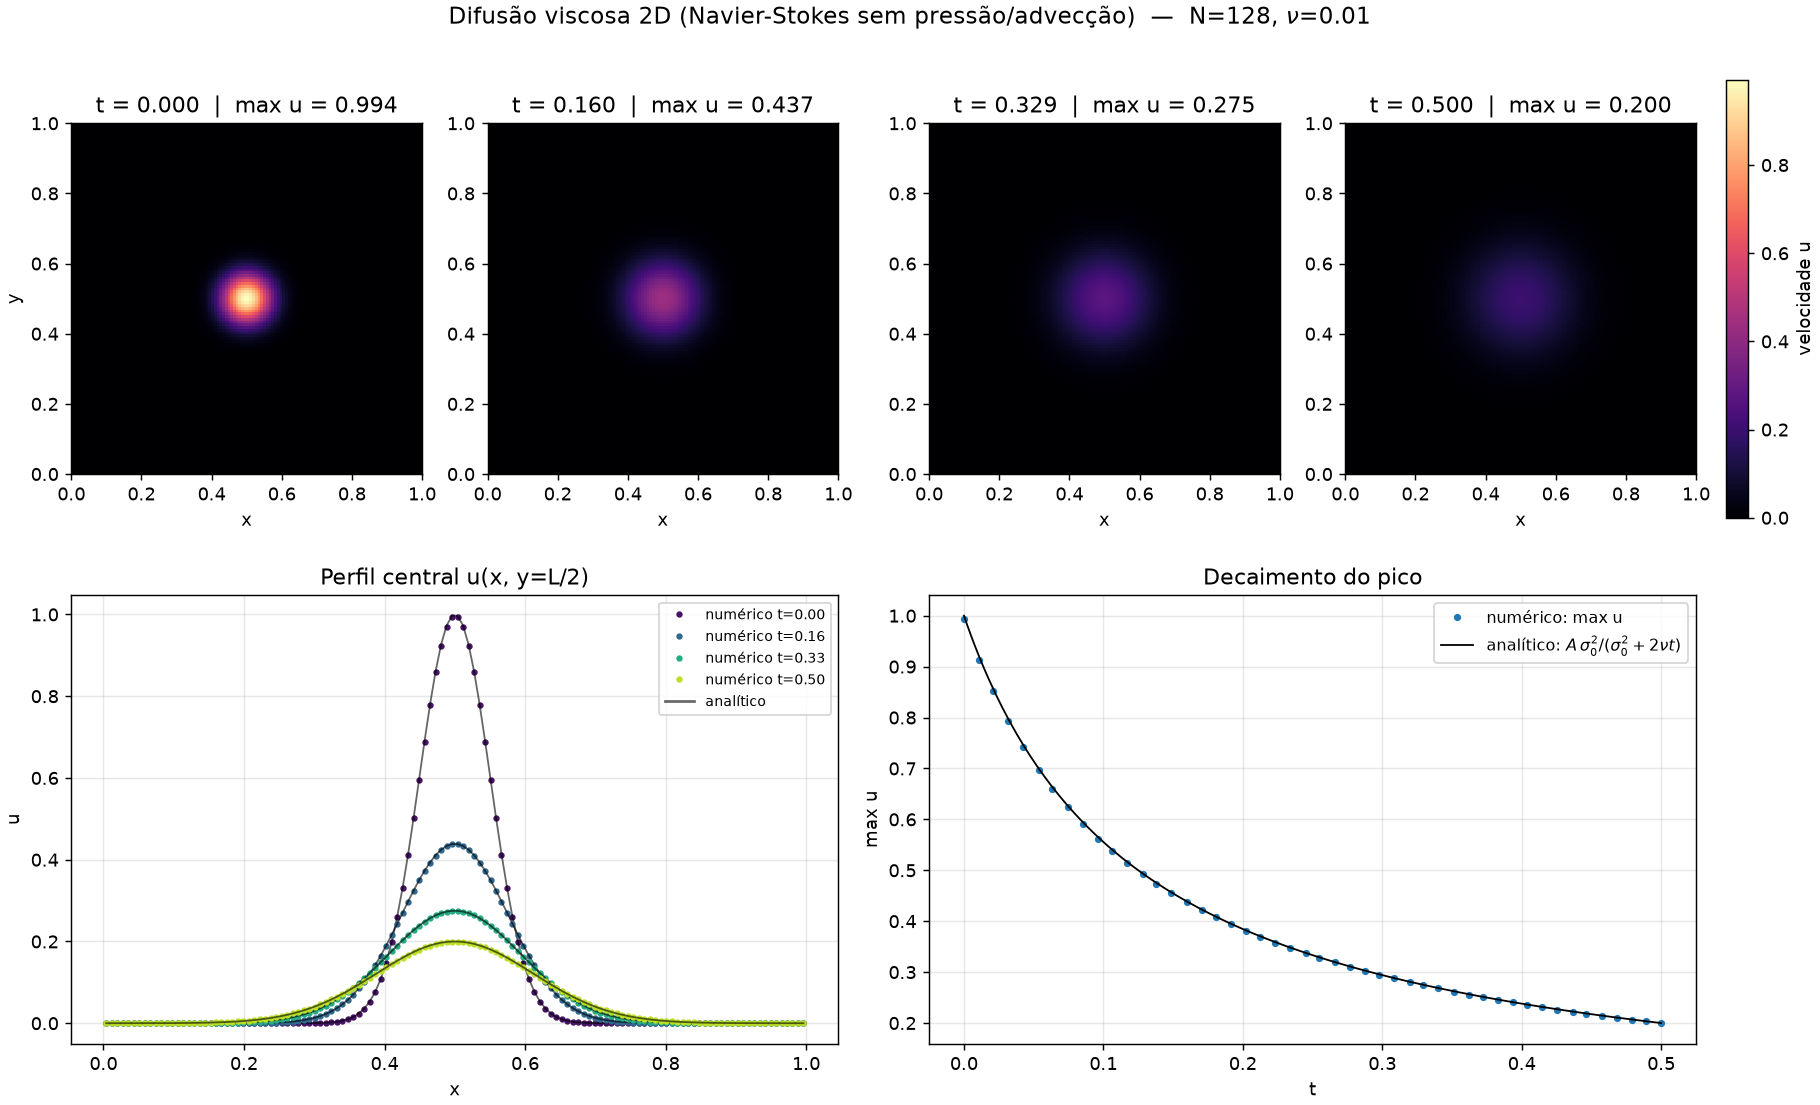
\includegraphics[width=\linewidth]{../ground_truth/simulacao1/difusao_figura.png}
    \caption{Difusão da perturbação gaussiana ($N=128$, $\nu = 0{,}01$),
    comparada com a solução analítica.}
    \label{fig:sim1}
\end{figure}

Os dois testes indicam que a discretização está correta: o estado de repouso é
preservado, e a perturbação se difunde suavemente, em concordância com a
solução analítica. O restante do relatório trata da versão paralela.

\section{Paralelização: impacto de \texttt{schedule} e \texttt{collapse}}

\subsection{O que se esperava}

O kernel tem duas características que orientam a escolha das cláusulas. A
carga é \emph{uniforme}: todos os pontos custam o mesmo, e como 1024 é
divisível por 2, 4 e 8, o \texttt{static} já distribui o trabalho de forma
exata, de modo que \texttt{dynamic} ou \texttt{guided} só acrescentariam
overhead de escalonamento. Além disso, o laço faz poucas operações por byte
lido e escrito (quatro arrays de $1024^2$ \texttt{double}, ou 32~MB no total), e por isso
tende a ser limitado pela largura de banda de memória. Nesse cenário, o
\texttt{collapse} não traz ganho de balanceamento (o laço externo já tem 1024
iterações, muito mais que as threads) e acrescenta custo de instruções: o
cálculo dos índices e dos vizinhos periódicos a cada ponto e um laço interno
menos favorável às otimizações do compilador. Apenas a política \texttt{static}
foi medida; \texttt{dynamic} e \texttt{guided} não foram avaliadas.

\subsection{Resultados do PaScal Suite}

A Tabela~\ref{tab:tempo} traz os tempos de execução e a
Tabela~\ref{tab:efsp}, a eficiência e o speedup, ambos extraídos do PaScal
Viewer. As figuras~\ref{fig:heat-ef} e \ref{fig:heat-sp} mostram os mesmos dados
como mapas de calor (cada mapa tem escala própria; o speedup vai de 0 a 3 no
\texttt{static} e de 0 a 4 no \texttt{collapse}).

\begin{table}[ht]
\centering
\caption{Tempo de execução (s) por número de cores e entrada.}
\label{tab:tempo}
\small
\begin{tabular}{c rrrr c rrrr}
\toprule
 & \multicolumn{4}{c}{\texttt{schedule(static)}} & & \multicolumn{4}{c}{\texttt{collapse(2)}} \\
\cmidrule(lr){2-5} \cmidrule(lr){7-10}
Cores & i1 & i2 & i3 & i4 & & i1 & i2 & i3 & i4 \\
\midrule
1 & 0,741 & 1,486 & 3,008 & 5,878 & & 1,115 & 2,107 & 4,217 & 8,379 \\
2 & 0,541 & 1,032 & 2,084 & 4,021 & & 0,549 & 1,139 & 2,233 & 4,396 \\
4 & 0,317 & 0,632 & 1,252 & 2,478 & & 0,317 & 0,617 & 1,224 & 2,288 \\
8 & 0,265 & 0,523 & 1,055 & 1,980 & & 0,304 & 0,603 & 1,143 & 2,145 \\
\bottomrule
\end{tabular}
\end{table}

\begin{table}[ht]
\centering
\caption{Eficiência (\%) e speedup, cada um relativo ao 1 core da própria
versão.}
\label{tab:efsp}
\small
\begin{tabular}{c rrrr c rrrr}
\toprule
 & \multicolumn{4}{c}{\texttt{schedule(static)}} & & \multicolumn{4}{c}{\texttt{collapse(2)}} \\
\cmidrule(lr){2-5} \cmidrule(lr){7-10}
\multicolumn{10}{l}{\emph{Eficiência (\%)}} \\
Cores & i1 & i2 & i3 & i4 & & i1 & i2 & i3 & i4 \\
\midrule
2 & 68,5 & 72,0 & 72,2 & 73,1 & & 101,5 & 92,5 & 94,4 & 95,3 \\
4 & 58,5 & 58,8 & 60,1 & 59,3 & & 88,0 & 85,4 & 86,2 & 91,5 \\
8 & 34,9 & 35,5 & 35,7 & 37,1 & & 45,8 & 43,6 & 46,1 & 48,8 \\
\midrule
\multicolumn{10}{l}{\emph{Speedup}} \\
Cores & i1 & i2 & i3 & i4 & & i1 & i2 & i3 & i4 \\
\midrule
2 & 1,37 & 1,44 & 1,44 & 1,46 & & 2,03 & 1,85 & 1,89 & 1,91 \\
4 & 2,34 & 2,35 & 2,40 & 2,37 & & 3,52 & 3,42 & 3,45 & 3,66 \\
8 & 2,79 & 2,84 & 2,85 & 2,97 & & 3,67 & 3,49 & 3,69 & 3,91 \\
\bottomrule
\end{tabular}
\end{table}

\begin{figure}[ht]
\centering
\begin{subfigure}[t]{0.48\textwidth}
  \includegraphics[width=\linewidth]{Efficiency_static.png}
  \caption{\texttt{schedule(static)}}
\end{subfigure}\hfill
\begin{subfigure}[t]{0.48\textwidth}
  \includegraphics[width=\linewidth]{Efficiency_collapse.png}
  \caption{\texttt{collapse(2)}}
\end{subfigure}
\caption{Mapas de eficiência do PaScal Viewer (cores $\times$ entradas).}
\label{fig:heat-ef}
\end{figure}

\begin{figure}[ht]
\centering
\begin{subfigure}[t]{0.48\textwidth}
  \includegraphics[width=\linewidth]{Speedup_static.png}
  \caption{\texttt{schedule(static)}}
\end{subfigure}\hfill
\begin{subfigure}[t]{0.48\textwidth}
  \includegraphics[width=\linewidth]{Speedup_collapse.png}
  \caption{\texttt{collapse(2)}}
\end{subfigure}
\caption{Mapas de speedup do PaScal Viewer (escalas diferentes entre os mapas).}
\label{fig:heat-sp}
\end{figure}

\subsection{Leitura pelas métricas do Viewer}

Medido contra o próprio tempo serial, o \texttt{collapse(2)} parece escalar
muito melhor: com 2, 4 e 8 cores, o speedup médio sobre as quatro entradas é
1,92, 3,51 e 3,69, contra 1,43, 2,37 e 2,86 do \texttt{static}, e a eficiência
média é de 95,9\%, 87,8\% e 46,1\%, contra 71,4\%, 59,2\% e 35,8\%. Com 2 cores
e a entrada i1, a eficiência do \texttt{collapse} chega a 101,5\%, um resultado
ligeiramente superlinear.

A métrica de escalabilidade do Viewer reforça esse quadro, e seus valores
publicados são reproduzidos pela diferença
$E(p, i_k) - E(p, i_1)$ em pontos percentuais, em que a eficiência de
referência é limitada a 100\%. Essa fórmula é uma inferência a partir dos
números, e não a definição oficial da ferramenta. No \texttt{static}, a
eficiência cresce levemente com o tamanho da entrada (de $+0{,}3$ a $+4{,}6$ p.p.).
No \texttt{collapse}, ela cai com 2 cores ($-7{,}5$ a $-4{,}7$ p.p.) e só
volta a subir com 4 cores em i4 ($+3{,}6$ p.p.) e com 8 cores em i3 e i4 ($+0{,}3$ e
$+3{,}0$ p.p.), porque o ponto de partida do \texttt{collapse} (i1) já é muito
alto.

\subsection{Comparação em tempo absoluto}

O speedup de cada versão usa uma base diferente, e as bases são muito
diferentes: com 1 core, o \texttt{collapse} leva em média 44\% mais tempo que o
\texttt{static} (por exemplo, 8,379~s contra 5,878~s em i4). Parte do
``melhor speedup'' do \texttt{collapse} vem, portanto, de partir de um tempo
serial mais alto. A Tabela~\ref{tab:comum} usa uma referência comum: o speedup
de ambas as versões em relação ao tempo serial do \texttt{static}, que é a
melhor execução com 1 core.

\begin{table}[ht]
\centering
\caption{Tempo do \texttt{collapse} em relação ao \texttt{static} (média das
quatro entradas) e speedup/eficiência com referência comum (1 core do
\texttt{static}).}
\label{tab:comum}
\small
\begin{tabular}{c c cc cc}
\toprule
 & Tempo & \multicolumn{2}{c}{Speedup (ref.\ comum)} &
 \multicolumn{2}{c}{Eficiência (ref.\ comum)} \\
\cmidrule(lr){3-4} \cmidrule(lr){5-6}
Cores & $T_{col}/T_{stat}$ & \texttt{static} & \texttt{collapse} &
\texttt{static} & \texttt{collapse} \\
\midrule
1 & 1,44 & 1,00 & 0,70 & 100\% & 70\% \\
2 & 1,07 & 1,43 & 1,34 & 71,4\% & 66,7\% \\
4 & 0,97 & 2,37 & 2,44 & 59,1\% & 61,1\% \\
8 & 1,12 & 2,86 & 2,57 & 35,8\% & 32,1\% \\
\bottomrule
\end{tabular}
\end{table}

\begin{figure}[ht]
\centering
\begin{tikzpicture}
\begin{axis}[
  width=0.75\textwidth, height=6.5cm,
  xlabel={Número de cores}, ylabel={Tempo de execução (s)},
  xmode=log, log basis x=2,
  xtick={1,2,4,8}, xticklabels={1,2,4,8},
  ymin=0, grid=major, legend pos=north east, legend cell align=left]
\addplot[blue, mark=square*] coordinates {(1,5.878) (2,4.021) (4,2.478) (8,1.980)};
\addlegendentry{\texttt{schedule(static)}}
\addplot[red, mark=*] coordinates {(1,8.379) (2,4.396) (4,2.288) (8,2.145)};
\addlegendentry{\texttt{collapse(2)}}
\end{axis}
\end{tikzpicture}
\caption{Tempo de execução na maior entrada (i4).}
\label{fig:tempo}
\end{figure}

Com essa referência, o quadro muda. O \texttt{collapse} é mais lento com 2 cores
(7\% em média) e com 8 cores (12\%), e só fica ligeiramente à frente com 4 cores
(3\% em média, até 7,7\% em i4; a diferença é pequena e pode estar dentro da
variação entre execuções, que não foi medida). A menor marca de tempo de cada
entrada é sempre do \texttt{static} com 8 cores (por exemplo, 1,980~s contra
2,145~s em i4).

\subsection{Interpretação}

\paragraph{Por que o \texttt{collapse} escala ``melhor'' sem ser mais rápido.}
O \texttt{collapse} faz mais trabalho por ponto: quatro comparações de contorno
por ponto, no lugar de duas por ponto mais duas por linha, a recuperação dos índices $i$ e
$j$ a partir do índice linear e um laço interno menos favorável à otimização do
compilador. Com 1 core, esse custo extra fica totalmente exposto (+44\% de
tempo). Com mais cores, o gargalo passa a ser a memória, e a computação
adicional é parcialmente escondida atrás das esperas por dados. O tempo do
\texttt{collapse} se aproxima do \texttt{static} (igual com 4 cores) e, ao
dividir pelo tempo serial mais alto, o speedup e a eficiência saem inflados.
Esse comportamento é compatível com um kernel limitado por memória, mas essa é
uma hipótese que os dados sustentam, e não uma medição direta.

\paragraph{O platô com 8 cores.} Entre 4 e 8 cores, o \texttt{static} ainda
reduz o tempo em 16\% a 20\%, enquanto o \texttt{collapse} reduz apenas 2\% a
7\%. Dobrar os cores não chega nem perto de dobrar o desempenho em nenhuma das
versões (eficiência de 36\% e 46\% com 8 cores). A causa exata do platô mais
marcado do \texttt{collapse} não foi determinada; entre as hipóteses estão a
saturação da largura de banda de memória, o compartilhamento de unidades de
execução se alguns dos 8 cores forem threads de hyper-threading, e o custo
adicional de instruções do \texttt{collapse}. Distinguir entre elas exigiria
os contadores de hardware (opção \texttt{--fgpe} do Analyzer) e a topologia da
máquina.

\paragraph{Balanceamento de carga.} Como a carga por ponto é uniforme e 1024 e
$1024^2$ são divisíveis por 2, 4 e 8, o desbalanceamento não explica a
diferença entre as versões. É coerente com isso o fato de a eficiência de cada
versão variar pouco entre as entradas i1 a i4 (poucos pontos percentuais),
isto é, o comportamento depende pouco do tamanho da simulação.

\paragraph{Sobre a cláusula \texttt{schedule}.} Neste problema, o
\texttt{schedule(static)} é a escolha natural: não há custo de escalonamento em
tempo de execução, e cada thread processa sempre o mesmo bloco de linhas em
todos os passos de tempo, o que favorece o reaproveitamento de cache e a
localidade em memória. Como a carga é uniforme, não há desbalanceamento que
\texttt{dynamic} ou \texttt{guided} pudessem corrigir; elas só adicionariam
overhead. Essa expectativa teórica não foi testada, pois apenas \texttt{static}
foi medido.

\subsection{Limitações}

\begin{itemize}
    \item Apenas \texttt{schedule(static)} foi medido, com e sem
    \texttt{collapse}; \texttt{dynamic}, \texttt{guided} e diferentes tamanhos
    de chunk ficaram de fora.
    \item Os tempos não trazem desvio padrão; as diferenças de poucos
    por cento (por exemplo, \texttt{collapse} 3\% mais rápido com 4 cores)
    podem estar dentro do ruído.
    \item O teste foi limitado a 8 cores, e as causas do platô com 8 cores são
    hipóteses não verificadas.
    \item Os mapas de escalabilidade forte e fraca, e a perda de speedup, não
    foram usados quantitativamente.
\end{itemize}

\section{Conclusão}

A simulação reproduz o comportamento esperado da difusão viscosa: o fluido
parado permanece parado, e uma perturbação gaussiana se alarga e perde
intensidade de acordo com a solução analítica, com o pico decaindo como
$A\sigma_0^2/(\sigma_0^2 + 2\nu t)$. Quanto à paralelização, o
\texttt{collapse(2)} parece escalar melhor nas métricas do Viewer (eficiência
de 95,9\% contra 71,4\% com 2 cores), mas esse resultado é em boa parte efeito
de um tempo serial 44\% maior. Em tempo absoluto, o \texttt{schedule(static)}
aplicado apenas ao laço externo é equivalente ou melhor em todas as contagens
de cores, exceto por uma pequena vantagem do \texttt{collapse} com 4 cores, e
obtém o menor tempo com 8 cores (speedup de 2,86 contra 2,57, com referência
comum). Para um laço externo com 1024 iterações e carga uniforme, o
\texttt{collapse} não traz benefício de balanceamento e acrescenta custo de
instruções. Ambas as versões apresentam eficiência baixa com 8 cores (36\% e
46\%), o que é consistente com um kernel limitado por memória.

Em resumo, métricas relativas ao próprio tempo serial devem ser lidas junto
com os tempos absolutos antes de se concluir qual cláusula é melhor.

\newpage
\appendix

\section{Código-fonte dos kernels}
\label{ap:codigo}

Os trechos a seguir são o passo de tempo das duas versões avaliadas. A
compilação foi feita com \texttt{gcc -O2 -Wall -fopenmp ... -lm -lmpascalops}.

\begin{lstlisting}[style=cstyle, caption={Versão \texttt{schedule}: paralelismo apenas no laço externo}, label={lst:sched}]
#define IDX(i, j, N) ((i) * (N) + (j))

static void passo(const double *u, const double *v,
                  double *un, double *vn, int N, double r)
{
    pascal_start(1);
    #pragma omp parallel for schedule(runtime)
    for (int i = 0; i < N; i++) {
        int im = (i == 0)     ? N - 1 : i - 1;
        int ip = (i == N - 1) ? 0     : i + 1;
        for (int j = 0; j < N; j++) {
            int jm = (j == 0)     ? N - 1 : j - 1;
            int jp = (j == N - 1) ? 0     : j + 1;

            double lap_u = u[IDX(ip, j, N)] + u[IDX(im, j, N)]
                         + u[IDX(i, jp, N)] + u[IDX(i, jm, N)]
                         - 4.0 * u[IDX(i, j, N)];
            double lap_v = v[IDX(ip, j, N)] + v[IDX(im, j, N)]
                         + v[IDX(i, jp, N)] + v[IDX(i, jm, N)]
                         - 4.0 * v[IDX(i, j, N)];

            un[IDX(i, j, N)] = u[IDX(i, j, N)] + r * lap_u;
            vn[IDX(i, j, N)] = v[IDX(i, j, N)] + r * lap_v;
        }
    }
    pascal_stop(1);
}
\end{lstlisting}

\begin{lstlisting}[style=cstyle, caption={Versão \texttt{collapse}: laços \texttt{i} e \texttt{j} fundidos}, label={lst:coll}]
static void passo(const double *u, const double *v,
                  double *un, double *vn, int N, double r)
{
    pascal_start(1);
    #pragma omp parallel for collapse(2) schedule(static)
    for (int i = 0; i < N; i++) {
        for (int j = 0; j < N; j++) {
            int im = (i == 0)     ? N - 1 : i - 1;
            int ip = (i == N - 1) ? 0     : i + 1;
            int jm = (j == 0)     ? N - 1 : j - 1;
            int jp = (j == N - 1) ? 0     : j + 1;

            double lap_u = u[IDX(ip, j, N)] + u[IDX(im, j, N)]
                         + u[IDX(i, jp, N)] + u[IDX(i, jm, N)]
                         - 4.0 * u[IDX(i, j, N)];
            double lap_v = v[IDX(ip, j, N)] + v[IDX(im, j, N)]
                         + v[IDX(i, jp, N)] + v[IDX(i, jm, N)]
                         - 4.0 * v[IDX(i, j, N)];

            un[IDX(i, j, N)] = u[IDX(i, j, N)] + r * lap_u;
            vn[IDX(i, j, N)] = v[IDX(i, j, N)] + r * lap_v;
        }
    }
    pascal_stop(1);
}
\end{lstlisting}

\end{document}